\documentclass{beamer}
% Use DS9 global theme (includes pgfplots for visualization)
\usepackage{../../../shared/templates/ds9_theme}

% Title page configuration
\title[Short Title]{PHYS12 CH:2.1-2.8 and 3.1-3.5}
\subtitle{Kinematics in One and Two Dimensions}
\author[Mr. Gullo]{Mr. Gullo}
\date[Sep 12, 2025]{September 12, 2025}

\begin{document}

\frame{\titlepage}

\begin{frame}
\frametitle{Learning Objectives}
\begin{columns}[T]
    \begin{column}{0.5\textwidth}
        \textbf{1D Kinematics:}
        \begin{itemize}
            \item Define position, displacement, distance, velocity, speed, and acceleration.
            \item Distinguish between scalar and vector quantities.
            \item Interpret graphs of position, velocity, and acceleration vs. time.
            \item Use kinematic equations to solve problems for objects with constant acceleration.
            \item Describe the motion of objects in free fall.
        \end{itemize}
    \end{column}
    \begin{column}{0.5\textwidth}
        \textbf{2D Kinematics:}
        \begin{itemize}
            \item Understand the independence of horizontal and vertical motions.
            \item Add and subtract vectors graphically and analytically.
            \item Resolve vectors into perpendicular components.
            \item Apply kinematic equations to solve projectile motion problems.
            \item Use vector addition to solve relative velocity problems.
        \end{itemize}
    \end{column}
\end{columns}
\end{frame}

\begin{frame}
\frametitle{From Physics 11 to Physics 12}
\begin{block}{Building on Foundations}
This course builds directly upon the concepts you learned in Physics 11. We'll quickly review Chapter 2 (1D kinematics) and extend to 2D motion.
\end{block}

\begin{columns}[T]
    \begin{column}{0.5\textwidth}
        \alert{From Chapter 2 (1D)}
        \begin{itemize}
            \item<2-> Position, displacement, distance
            \item<3-> Scalars vs. vectors (+/- directions)
            \item<4-> Kinematic equations for constant acceleration
            \item<5-> Free fall and graphical analysis
        \end{itemize}
    \end{column}
    \begin{column}{0.5\textwidth}
        \alert{New in 2D}
        \begin{itemize}
            \item<2-> Vector components and trigonometry
            \item<3-> Independence of horizontal/vertical motion
            \item<4-> Projectile motion analysis
            \item<5-> Relative velocity problems
        \end{itemize}
    \end{column}
\end{columns}
\end{frame}

\section{1D Kinematics Review}

\begin{frame}
\frametitle{Reference to Chapter 2: 1D Kinematics}
\framesubtitle{Foundation for 2D Motion}
\begin{block}{Quick Reference}
For detailed explanations of 1D kinematics concepts, see \textbf{Chapter 2 slides}:
\begin{itemize}
    \item Position, displacement, and distance
    \item Scalars vs. vectors with detailed examples
    \item Full derivation of kinematic equations
    \item Free fall motion and analysis
    \item Graphical analysis with worked examples
    \item GUESS method for problem solving
\end{itemize}
\end{block}
\begin{alertblock}{This Chapter}
We'll focus on extending these concepts to 2D motion using vector components!
\end{alertblock}
\end{frame}

\begin{frame}
\frametitle{1D Kinematics: Essential Review}
\framesubtitle{Building on Chapter 2 Foundations}
\begin{block}{Core Concepts (From Chapter 2)}
\begin{itemize}
    \item \textbf{Position vs. Displacement}: $\Delta x = x_f - x_0$ (vector)
    \item \textbf{Distance}: Total path length (scalar, always positive)
    \item \textbf{Velocity}: $\bar{v} = \Delta x / \Delta t$ (vector)
    \item \textbf{Speed}: Distance/time (scalar)
    \item \textbf{Acceleration}: $\bar{a} = \Delta v / \Delta t$ (vector)
\end{itemize}
\end{block}
\alert{Key 2D Extension}: In 1D, direction was simple (+ or -). In 2D, we need full vector mathematics!
\end{frame}

\begin{frame}
\frametitle{Vectors in 1D vs. 2D: Quick Review}
\framesubtitle{From Simple Signs to Full Components}
\begin{columns}[T]
    \begin{column}{0.5\textwidth}
        \alert{1D Motion (Chapter 2)}
        \begin{itemize}
            \item Direction: + or - sign
            \item Example: $v = +5$ m/s or $v = -3$ m/s
            \item Vector addition: Simple algebra
        \end{itemize}
    \end{column}
    \begin{column}{0.5\textwidth}
        \alert{2D Motion (This Chapter)}
        \begin{itemize}
            \item Direction: Angle and magnitude
            \item Example: $\vec{v} = 5$ m/s at 30°
            \item Vector addition: Components needed
        \end{itemize}
    \end{column}
\end{columns}
\vspace{1em}
\begin{block}{Why This Matters}
In 2D, we can't just use + and - to represent all possible directions. We need trigonometry and vector components!
\end{block}
\end{frame}

\begin{frame}
\frametitle{Acceleration: Quick Review}
\framesubtitle{The Bridge to 2D Motion}
\begin{block}{From Chapter 2}
\begin{itemize}
    \item \textbf{Acceleration}: Rate of velocity change, $\bar{a} = \Delta v / \Delta t$
    \item \textbf{Key Insight}: In 2D, acceleration can change speed, direction, or both!
    \item \textbf{Free Fall}: $a = -g = -9.80$ m/s² (constant downward)
\end{itemize}
\end{block}
\begin{alertblock}{2D Challenge}
How do we handle acceleration that's not aligned with our motion direction? This is where vector components become essential!
\end{alertblock}
\end{frame}

\section{Kinematic Equations: Quick Reference}

\begin{frame}
\frametitle{Kinematic Equations: Review and Extension}
\framesubtitle{From 1D to 2D Applications}
\begin{block}{The Four Equations (From Chapter 2)}
For constant acceleration only:
\begin{align*}
    v_f &= v_0 + at \\
    \Delta x &= \frac{1}{2}(v_0 + v_f)t \\
    \Delta x &= v_0 t + \frac{1}{2}at^2 \\
    v_f^2 &= v_0^2 + 2a\Delta x
\end{align*}
\end{block}
\begin{alertblock}{2D Strategy}
We'll apply these equations \textbf{separately} to x and y components!
\end{alertblock}
\end{frame}

\section{Free Fall: Review and 2D Extension}

\begin{frame}
\frametitle{Free Fall: Essential Concepts}
\framesubtitle{Building on Chapter 2 for Projectile Motion}
\begin{block}{Key Review (From Chapter 2)}
\begin{itemize}
    \item \textbf{Free Fall}: Motion under gravity only ($a = -g = -9.80$ m/s²)
    \item \textbf{Sign Convention}: Up = positive, so $a_y = -9.80$ m/s²
    \item \textbf{Key Insight}: All objects fall at same rate (neglecting air resistance)
\end{itemize}
\end{block}
\begin{alertblock}{2D Application}
In projectile motion, only the \textbf{vertical component} follows free fall. The \textbf{horizontal component} has no acceleration!
\end{alertblock}
\end{frame}

\begin{frame}
\frametitle{Free Fall Graphs: Quick Review}
\framesubtitle{Essential Patterns for Projectile Motion}
\begin{columns}[T]
    \begin{column}{0.33\textwidth}
        \textbf{Position vs. Time}
        \begin{itemize}
            \item Parabolic shape
            \item Slope = velocity
        \end{itemize}
    \end{column}
    \begin{column}{0.33\textwidth}
        \textbf{Velocity vs. Time}
        \begin{itemize}
            \item Straight line
            \item Slope = $-g$
            \item Area = $\Delta y$
        \end{itemize}
    \end{column}
    \begin{column}{0.33\textwidth}
        \textbf{Acceleration vs. Time}
        \begin{itemize}
            \item Constant: $-g$
            \item Always downward
        \end{itemize}
    \end{column}
\end{columns}
\vspace{1em}
\begin{block}{2D Connection}
These same patterns apply to the \textbf{vertical component} of projectile motion!
\end{block}
\end{frame}

\section{Graphical Analysis: Essential Review}

\begin{frame}
\frametitle{Motion Graphs: Key Relationships}
\framesubtitle{Quick Review from Chapter 2}
\begin{columns}[T]
    \begin{column}{0.5\textwidth}
        \textbf{Position-Time Graph}
        \begin{itemize}
            \item \alert{Slope} = velocity
            \item Curved = acceleration
            \item Steeper = faster
        \end{itemize}
    \end{column}
    \begin{column}{0.5\textwidth}
        \textbf{Velocity-Time Graph}
        \begin{itemize}
            \item \alert{Slope} = acceleration
            \item \alert{Area} = displacement
            \item Horizontal = constant velocity
        \end{itemize}
    \end{column}
\end{columns}
\vspace{1em}
\begin{block}{2D Application}
We'll analyze x and y components separately using these same principles!
\end{block}
\end{frame}

\section{1D Problem Solving: Quick Reference}

\begin{frame}
\frametitle{Problem Solving: GUESS Method Review}
\framesubtitle{From Chapter 2 to 2D Applications}
\begin{block}{The GUESS Method (Chapter 2)}
\begin{itemize}
    \item \textbf{G} - \alert{Givens}: List known quantities, define coordinate system
    \item \textbf{U} - \alert{Unknown}: Identify what to find
    \item \textbf{E} - \alert{Equation}: Choose appropriate kinematic equation
    \item \textbf{S} - \alert{Substitute}: Plug in values with units
    \item \textbf{S} - \alert{Solve}: Calculate and check units/significant figures
\end{itemize}
\end{block}
\begin{alertblock}{2D Extension}
For 2D problems: Apply GUESS \textbf{separately} to x and y components!
\end{alertblock}
\end{frame}

\part{Part 2: Two-Dimensional Kinematics}
\section{2D Motion Concepts}

\begin{frame}
\frametitle{2D Motion: The Independence of Motion}
\begin{block}{The Most Important Concept in 2D Kinematics}
The horizontal and vertical components of two-dimensional motion are \textbf{independent} of each other.
\end{block}
\begin{itemize}
    \item Motion in the horizontal direction does not affect motion in the vertical direction, and vice versa.
    \item This allows us to break complex 2D problems into two simpler 1D problems: one for the x-direction and one for the y-direction.
    \item The only variable that connects the two separate motions is \alert{time ($t$)}.
\end{itemize}
\end{frame}

\begin{frame}
\frametitle{Concept Visualization: Independence of Motion (Context)}
\begin{block}{Scenario: The Two-Ball Drop}
Imagine two identical balls at the same height.
\begin{itemize}
    \item Ball 1 is dropped straight down.
    \item Ball 2 is launched horizontally at the exact same moment.
\end{itemize}
\textbf{Question:} Which ball hits the ground first?
\end{block}
Let's visualize their motion. The result demonstrates the independence of vertical and horizontal motion.
\end{frame}

\begin{frame}
\frametitle{Concept Visualization: Independence of Motion}
\begin{alertblock}{[Diagram based on Figure 3.6]}
A composite image showing the motion of two balls.
\begin{itemize}
    \item The red ball is dropped vertically from rest.
    \item The blue ball is projected horizontally with an initial velocity.
    \item Strobe flashes at equal time intervals show that both balls have the same vertical position at any given moment.
    \item This demonstrates that the horizontal motion of the blue ball does not affect its vertical motion due to gravity. They hit the ground at the same time.
\end{itemize}
\end{alertblock}
\end{frame}

\begin{frame}
\frametitle{Visualization: Dropped vs. Fired Ball Experiment}
\begin{center}
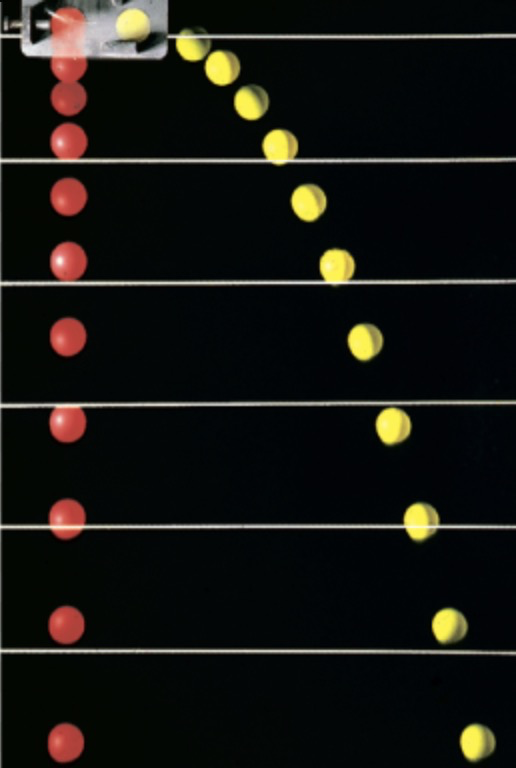
\includegraphics[width=0.8\linewidth]{phys12-projectile-motion-trajectory-analysis.png}
\end{center}
\begin{block}{Key Observation}
The strobe images show both balls at the same vertical positions at each time interval, demonstrating that horizontal motion does not affect vertical motion under gravity.
\end{block}
\end{frame}

\section{Vectors in 2D}

\begin{frame}
\frametitle{Vector Addition: Head-to-Tail Method}
\begin{block}{Graphical Method for Adding Vectors}
To add vectors graphically, we draw them one after another.
\end{block}
\begin{enumerate}
    \item Draw the first vector to scale and in the correct direction.
    \item Draw the second vector starting from the head (tip) of the first vector.
    \item Continue for all vectors.
    \item The \textbf{resultant vector} ($\vec{R}$) is the vector drawn from the tail (start) of the first vector to the head of the last vector.
\end{enumerate}
\vfill
\begin{alertblock}{[Diagram illustrating the head-to-tail method for adding vectors $\vec{A}$ and $\vec{B}$, showing the resultant vector $\vec{R}$. Based on Figure 3.10]}
\end{alertblock}
\end{frame}

\begin{frame}
\frametitle{Visualization: Vector Addition Example}
\begin{center}
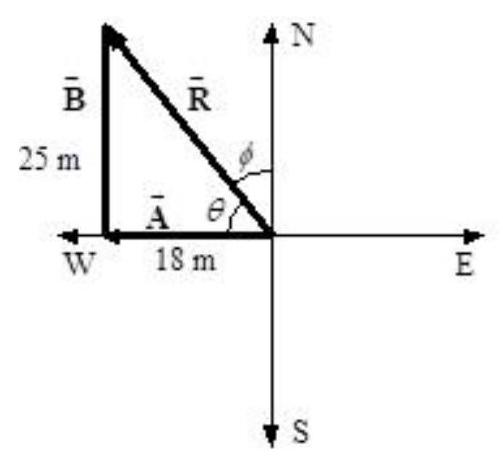
\includegraphics[width=0.7\linewidth]{phys12-vectors-vector-addition-figure-4.png}
\end{center}
\begin{block}{Key Observation}
The resultant vector $\vec{R} = \vec{A} + \vec{B}$ is drawn from the tail of the first vector to the head of the second vector.
\end{block}
\end{frame}

\begin{frame}
\frametitle{Analytical Method: Vector Components}
\begin{block}{Using Trigonometry for Precision}
Any 2D vector can be broken down into two perpendicular components. We typically use x and y axes.
\end{block}
\begin{itemize}
    \item For a vector $\vec{A}$ with magnitude $A$ and at an angle $\theta$ (measured from the positive x-axis):
    \begin{itemize}
        \item The x-component is $A_x = A \cos \theta$
        \item The y-component is $A_y = A \sin \theta$
    \end{itemize}
    \item This process is called \textbf{resolving the vector}.
    \item To add vectors $\vec{A}$ and $\vec{B}$ to get $\vec{R}$:
    \begin{itemize}
        \item Add the x-components: $R_x = A_x + B_x$
        \item Add the y-components: $R_y = A_y + B_y$
    \end{itemize}
    \item Then, find the magnitude and direction of $\vec{R}$ using its components.
\end{itemize}
\end{frame}

\begin{frame}
\frametitle{Advanced Topic: Rotated Coordinate Systems}
\begin{columns}
\column{0.6\textwidth}
\begin{block}{When Axes Are Rotated}
Sometimes we need to resolve vectors along axes that are not aligned with the standard x-y coordinate system.
\begin{itemize}
    \item Common in navigation and engineering
    \item The trigonometric principles remain the same
    \item Adjust angles relative to the new axes
\end{itemize}
\end{block}

\column{0.4\textwidth}
\begin{figure}
\centering
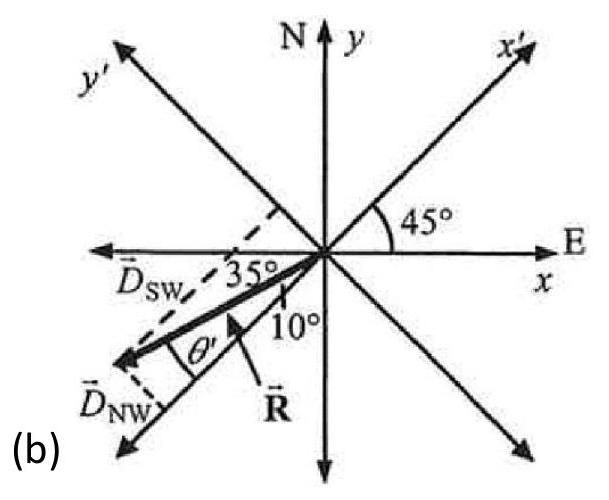
\includegraphics[width=0.9\textwidth]{phys12-vectors-vector-addition-figure-21.png}
\caption{Vector components along rotated axes}
\end{figure}
\end{columns}
\end{frame}

\begin{frame}
\frametitle{Concept Visualization: Vector Components (Context)}
\begin{block}{Breaking a Vector Apart}
Let's visualize how a single vector $\vec{A}$ can be represented as the sum of its perpendicular components, $\vec{A}_x$ and $\vec{A}_y$.
\vfill
This is the reverse of adding vectors and is a crucial first step for solving almost any 2D physics problem.
\end{block}
\end{frame}

\begin{frame}
\frametitle{Concept Visualization: Vector Components}
\begin{columns}
\column{0.5\textwidth}
\begin{figure}
\begin{tikzpicture}[scale=1.5, thick]
    % Axes
    \draw[->] (0,0) -- (4,0) node[below] {$x$};
    \draw[->] (0,0) -- (0,3) node[left] {$y$};

    % Vector A
    \draw[->, ds9blue, line width=1.5pt] (0,0) -- (3,2) node[midway, above left] {$\vec{A}$};
    \draw (0.5,0) arc (0:33.7:0.5) node[midway, right] {$\theta$};

    % Components
    \draw[->, ds9red, dashed, line width=1.2pt] (0,0) -- (3,0) node[midway, below] {$A_x = A \cos\theta$};
    \draw[->, ds9red, dashed, line width=1.2pt] (3,0) -- (3,2) node[midway, right] {$A_y = A \sin\theta$};

    % Right angle
    \draw (2.7,0) -- (2.7,0.3) -- (3,0.3);
\end{tikzpicture}
\caption{Mathematical representation of vector components}
\end{figure}

\column{0.5\textwidth}
\begin{figure}
\centering
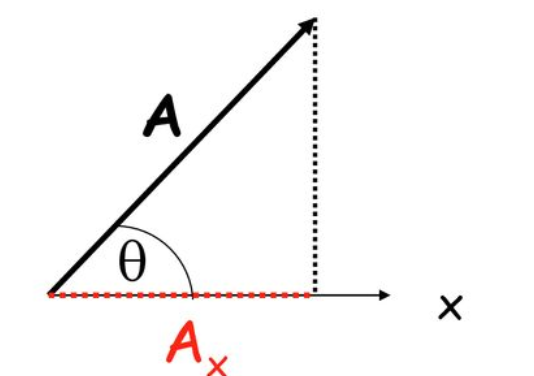
\includegraphics[width=0.8\textwidth]{phys12-vectors-vector-components.png}
\caption{Alternative visualization of vector components}
\end{figure}
\end{columns}
\end{frame}

\begin{frame}
\frametitle{Trigonometry Reference for Vector Components}
\begin{columns}[T]
    \column{0.48\textwidth}
    \begin{figure}
        \centering
        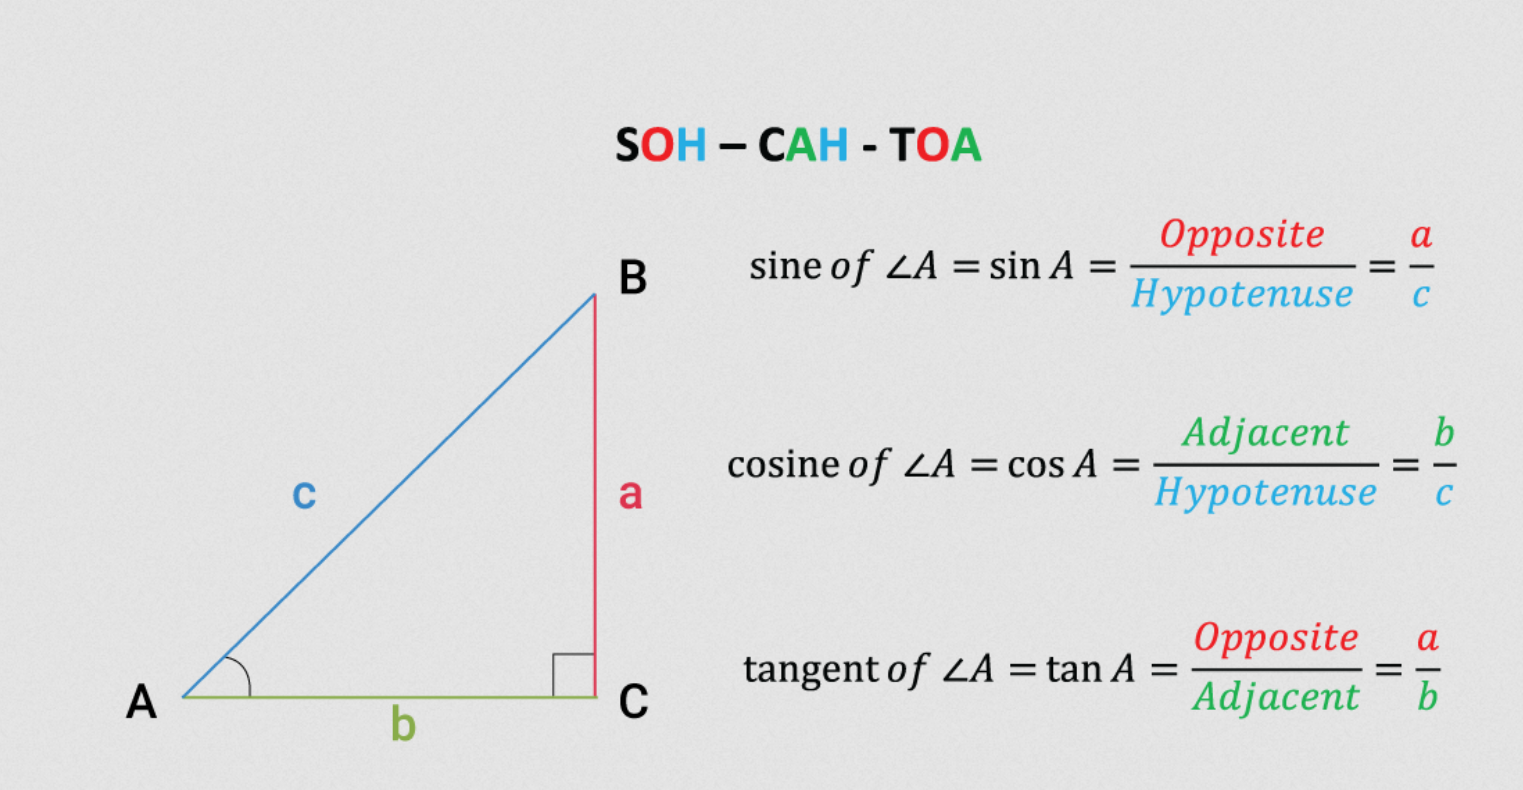
\includegraphics[width=\linewidth]{math-trigonometry-sohcahtoa.png}
        \caption{SOHCAHTOA mnemonic for finding vector components}
    \end{figure}

    \column{0.48\textwidth}
    \begin{figure}
        \centering
        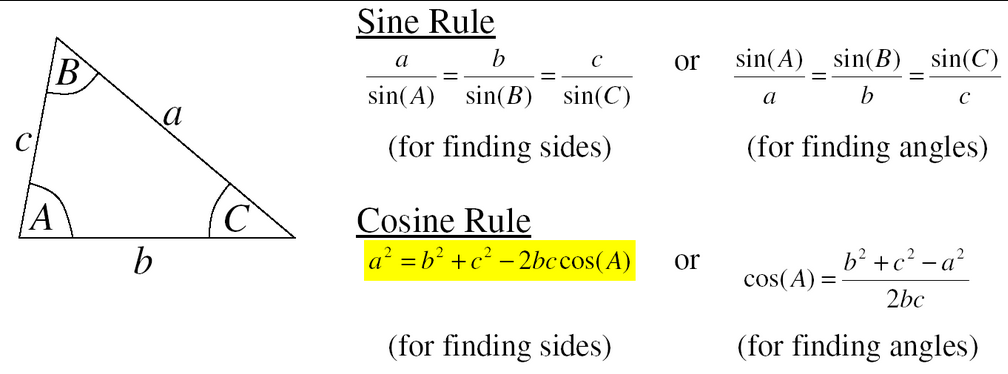
\includegraphics[width=\linewidth]{math-sine-cosine-laws.png}
        \caption{Sine and cosine laws for non-right triangles}
    \end{figure}
\end{columns}
\begin{block}{Key Applications}
These trigonometric relationships are essential for:
\begin{itemize}
    \item Resolving vectors into components
    \item Finding magnitude and direction from components
    \item Solving vector addition problems
\end{itemize}
\end{block}
\end{frame}

\section{Projectile Motion}

\begin{frame}
\frametitle{Key Concepts: Projectile Motion}
\begin{block}{Applying 2D Kinematics}
A \textbf{projectile} is any object that is thrown or launched and then moves subject only to gravity.
\end{block}
\textbf{Analysis Steps:}
\begin{enumerate}
    \item Set up a coordinate system (usually origin at launch, +y is up).
    \item Resolve the initial velocity ($v_0$) into components:
    \begin{itemize}
        \item $v_{0x} = v_0 \cos \theta_0$
        \item $v_{0y} = v_0 \sin \theta_0$
    \end{itemize}
    \item Treat as two independent 1D motion problems:
    \begin{itemize}
        \item \textbf{Horizontal (x):} Constant velocity ($a_x = 0$)
        \item \textbf{Vertical (y):} Constant acceleration ($a_y = -g$)
    \end{itemize}
    \item Use the kinematic equations for each direction. Time ($t$) is the same for both.
\end{enumerate}
\end{frame}

\section{Relative Velocity}

\begin{frame}
\frametitle{Key Concepts: Relative Velocity}
\begin{block}{Motion Depends on the Observer}
Velocity is always measured \textit{relative} to a frame of reference.
\end{block}
\begin{itemize}
    \item The velocity of an object can have different values when measured by different observers.
    \item We use vector addition to find the velocity of an object relative to a stationary observer (e.g., the ground).
    \item \textbf{Subscript Notation} is very helpful:
    \begin{itemize}
        \item $\vec{v}_{PG}$ = Velocity of the \textbf{P}lane relative to the \textbf{G}round.
        \item $\vec{v}_{PA}$ = Velocity of the \textbf{P}lane relative to the \textbf{A}ir.
        \item $\vec{v}_{AG}$ = Velocity of the \textbf{A}ir relative to the \textbf{G}round (i.e., the wind).
    \end{itemize}
    \item \textbf{Relative Velocity Equation}: $\vec{v}_{PG} = \vec{v}_{PA} + \vec{v}_{AG}$
\end{itemize}
\end{frame}

\begin{frame}
\frametitle{Visualization: Train Relative Velocity Example}
\begin{center}
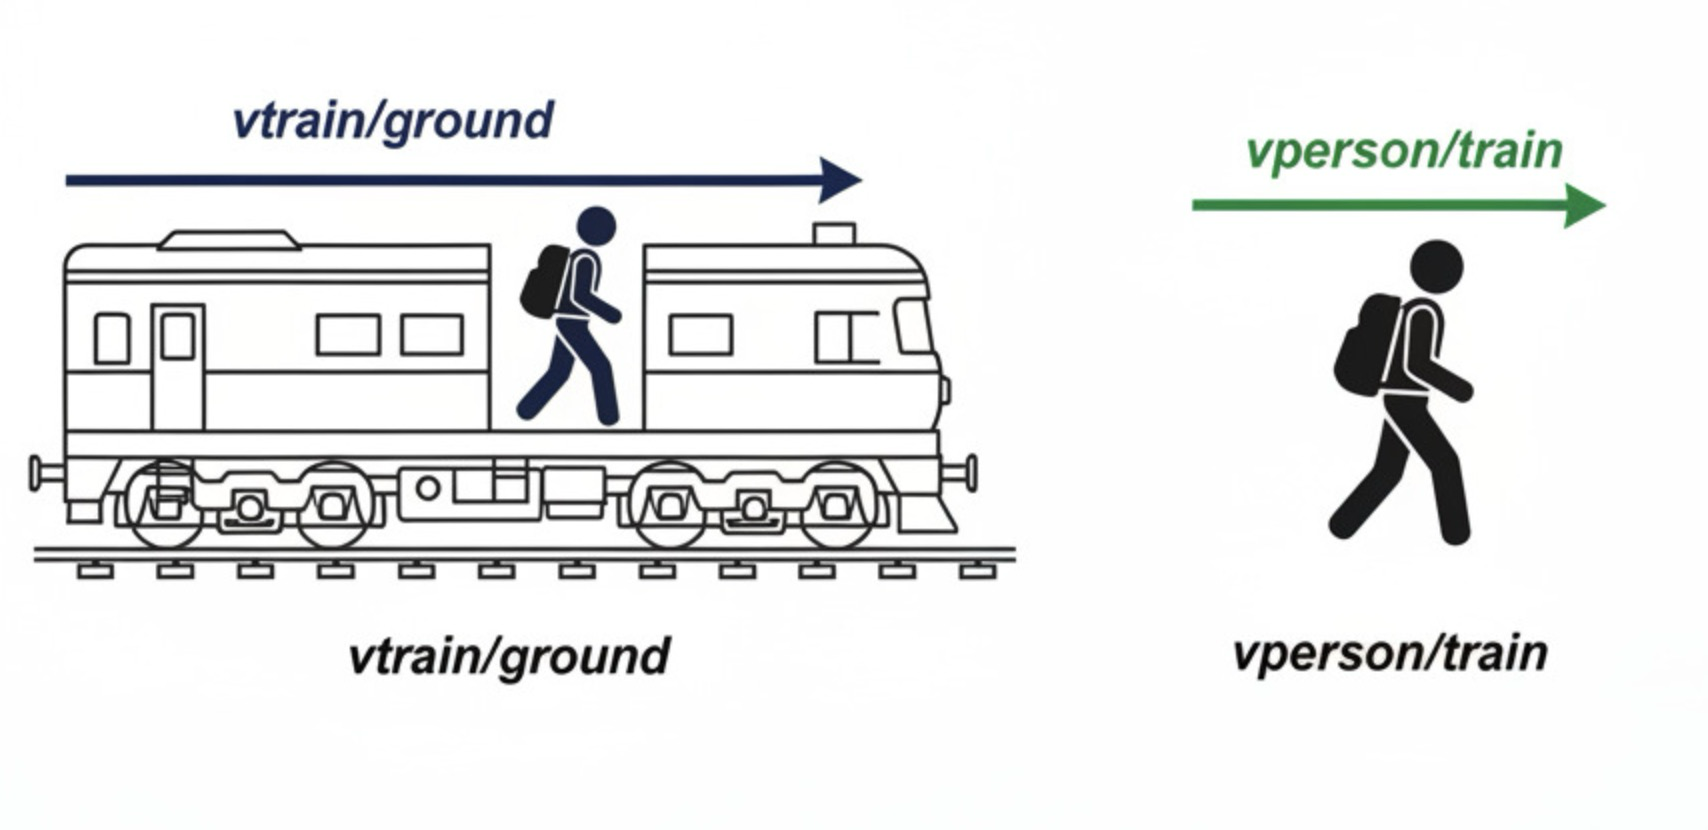
\includegraphics[width=0.8\linewidth]{phys12-relative-velocity-train.png}
\end{center}
\begin{block}{Understanding the Diagram}
\begin{itemize}
    \item The train moves with velocity $\vec{v}_{train/ground}$ relative to the ground
    \item The person walks with velocity $\vec{v}_{person/train}$ relative to the train
    \item The person's velocity relative to the ground is the vector sum: $\vec{v}_{person/ground} = \vec{v}_{person/train} + \vec{v}_{train/ground}$
\end{itemize}
\end{block}
\end{frame}

\begin{frame}
\frametitle{Concept Visualization: Boat in a River (Context)}
\begin{block}{Scenario: Crossing a Current}
A boat tries to travel straight across a river. However, the river's current carries the boat downstream.
\begin{itemize}
    \item $\vec{v}_{bw}$: Velocity of the \textbf{b}oat relative to the \textbf{w}ater.
    \item $\vec{v}_{wg}$: Velocity of the \textbf{w}ater relative to the \textbf{g}round (the current).
    \item $\vec{v}_{bg}$: Velocity of the \textbf{b}oat relative to the \textbf{g}round (its actual path).
\end{itemize}
The boat's actual velocity is the vector sum of its velocity in the water and the water's velocity.
\end{block}
\end{frame}

\begin{frame}
\frametitle{Concept Visualization: Boat in a River}
\begin{alertblock}{[Diagram based on Figure 3.40]}
A diagram showing a river with a current flowing to the right.
\begin{itemize}
    \item A vector labeled $\vec{v}_{bw}$ points straight across the river.
    \item A vector labeled $\vec{v}_{wg}$ points downstream, parallel to the banks.
    \item The resultant vector $\vec{v}_{bg} = \vec{v}_{bw} + \vec{v}_{wg}$ points diagonally downstream, showing the boat's true path relative to the ground.
\end{itemize}
\end{alertblock}
\end{frame}

\section{2D Problem Solving}

\begin{frame}
\frametitle{I do: Fireworks Projectile (Ex. 3.4)}
\begin{block}{Problem}
A firework is shot with an initial speed of 70.0 m/s at an angle of 75.0° above the horizontal. (a) Calculate the height at which it explodes (its apex). (b) How much time passes until it explodes?
\end{block}
\pause
\begin{columns}[T]
\column{0.48\textwidth}
\begin{block}{G - Givens}
\begin{itemize}
\item $v_0 = 70.0$ m/s
\item $\theta_0 = 75.0^\circ$
\item $y_0 = 0$ m, $x_0 = 0$ m
\item $a_y = -9.80$ m/s$^2$
\item $a_x = 0$ m/s$^2$
\item At apex: $v_{fy} = 0$ m/s
\end{itemize}
\end{block}
\pause
\column{0.48\textwidth}
\begin{block}{U - Unknown}
\begin{itemize}
\item (a) $y_f = ?$
\item (b) $t = ?$
\end{itemize}
\end{block}
\end{columns}
\end{frame}

\begin{frame}
\frametitle{I do: Fireworks Projectile (Ex. 3.4)}

\pause
\begin{columns}[T]
\column{0.48\textwidth}
\begin{block}{G - Givens}
\begin{itemize}
\item $v_0 = 70.0$ m/s
\item $\theta_0 = 75.0^\circ$
\item $y_0 = 0$ m, $x_0 = 0$ m
\item $a_y = -9.80$ m/s$^2$
\item $a_x = 0$ m/s$^2$
\item At apex: $v_{fy} = 0$ m/s
\end{itemize}
\end{block}
\pause
\column{0.48\textwidth}
\begin{block}{U - Unknown}
\begin{itemize}
\item (a) $y_f = ?$
\item (b) $t = ?$
\end{itemize}
\end{block}
\end{columns}
\pause
\begin{columns}[T]
\column{0.48\textwidth}
\begin{block}{E - Equation}
\begin{itemize}
\item $v_{0y} = v_0 \sin\theta_0$
\item $v_{fy}^2 = v_{0y}^2 + 2a_y\Delta y$
\item \textbf{Rearranged}: $y_f = y_0 + \frac{v_{fy}^2 - v_{0y}^2}{2a_y}$
\item $v_{fy} = v_{0y} + a_y t$
\item \textbf{Rearranged}: $t = \frac{v_{fy} - v_{0y}}{a_y}$
\end{itemize}
\end{block}
\end{columns}
\end{frame}

\begin{frame}
\frametitle{I do: Fireworks Projectile (Ex. 3.4)}

\begin{block}{S - Substitute}
\begin{itemize}
\item $v_{0y} = (70.0 \text{ m/s})\sin(75.0^\circ) = 67.6$ m/s
\item $y_f = 0 + \frac{(0)^2 - (67.6)^2}{2(-9.80)}$
\item $t = \frac{0 - 67.6}{-9.80}$
\end{itemize}
\end{block}
\pause
\begin{block}{S - Solve}
\begin{itemize}
\item $y_f = \frac{-4570}{-19.6} = 233$ m
\item $t = \frac{-67.6}{-9.80} = 6.90$ s
\item \boxed{y_f = 233 \text{ m}} and \boxed{t = 6.90 \text{ s}}
\end{itemize}
\end{block}
\end{frame}

\begin{frame}
\frametitle{We do: Hot Rock Projectile (Ex. 3.5)}
\begin{block}{Problem}
A rock is ejected from a volcano with speed 25.0 m/s at 35.0° above the horizontal. It strikes the side of the volcano 20.0 m \textit{lower} than its starting point. (a) Calculate the time it takes.
\end{block}
\pause
\begin{columns}[T]
\column{0.48\textwidth}
\begin{block}{G - Givens}
\begin{itemize}
\item $v_0 = 25.0$ m/s
\item $\theta_0 = 35.0^\circ$
\item $y_0 = 0$ m
\item $y_f = -20.0$ m
\item $a_y = -9.80$ m/s$^2$
\end{itemize}
\end{block}
\pause
\column{0.48\textwidth}
\begin{block}{U - Unknown}
\begin{itemize}
\item $t = ?$
\end{itemize}
\end{block}
\end{columns}
\end{frame}

\begin{frame}
\frametitle{We do: Hot Rock Projectile (Ex. 3.5)}
\pause
\begin{columns}[T]
\column{0.48\textwidth}
\begin{block}{G - Givens}
\begin{itemize}
\item $v_0 = 25.0$ m/s
\item $\theta_0 = 35.0^\circ$
\item $y_0 = 0$ m
\item $y_f = -20.0$ m
\item $a_y = -9.80$ m/s$^2$
\end{itemize}
\end{block}
\pause
\column{0.48\textwidth}
\begin{block}{U - Unknown}
\begin{itemize}
\item $t = ?$
\end{itemize}
\end{block}
\end{columns}
\pause
\begin{columns}[T]
\column{0.48\textwidth}
\begin{block}{E - Equation}
\begin{itemize}
\item $v_{0y} = v_0 \sin\theta_0$
\item $\Delta y = v_{0y}t + \frac{1}{2}a_y t^2$
\item \textbf{Rearranged}: $\frac{1}{2}a_y t^2 + v_{0y}t - \Delta y = 0$
\end{itemize}
\end{block}
\end{columns}
\end{frame}

\begin{frame}
\frametitle{We do: Hot Rock Projectile (Ex. 3.5)}

\begin{block}{S - Substitute}
\begin{itemize}
\item $v_{0y} = (25.0)\sin(35.0^\circ) = 14.3$ m/s
\item $\Delta y = -20.0 - 0 = -20.0$ m
\item $-20.0 = (14.3)t + \frac{1}{2}(-9.80)t^2$
\item $4.90t^2 - 14.3t - 20.0 = 0$
\end{itemize}
\end{block}
\pause
\begin{block}{S - Solve}
\begin{itemize}
\item $t = \frac{-b \pm \sqrt{b^2 - 4ac}}{2a}$
\item $a = 4.90$, $b = -14.3$, $c = -20.0$
\item $t = \frac{14.3 \pm \sqrt{204.49 + 392}}{9.80} = \frac{14.3 \pm 24.4}{9.80}$
\item $t = 3.95$ s
\item \boxed{t = 3.95 \text{ s}}
\end{itemize}
\end{block}
\end{frame}

\begin{frame}
\frametitle{You do: Projectile Launch}
\begin{block}{Problem (Ch.3, Q.25)}
A projectile is launched at ground level with an initial speed of 50.0 m/s at an angle of 30.0° above the horizontal. It strikes a target 3.00 seconds later.
\begin{enumerate}
    \item What is the horizontal distance ($x$) to the target?
    \item What is the vertical distance ($y$) to the target?
\end{enumerate}
\end{block}
\pause
\begin{columns}[T]
\column{0.48\textwidth}
\begin{block}{G - Givens}
\begin{itemize}
\item $v_0 = 50.0$ m/s
\item $\theta_0 = 30.0^\circ$
\item $x_0 = 0$ m, $y_0 = 0$ m
\item $t = 3.00$ s
\item $a_x = 0$ m/s$^2$
\item $a_y = -9.80$ m/s$^2$
\end{itemize}
\end{block}
\pause
\column{0.48\textwidth}
\begin{block}{U - Unknown}
\begin{itemize}
\item (a) $x_f = ?$
\item (b) $y_f = ?$
\end{itemize}
\end{block}
\end{columns}
\end{frame}

\begin{frame}
\frametitle{You do: Projectile Launch}


\begin{columns}[T]
\column{0.48\textwidth}
\begin{block}{G - Givens}
\begin{itemize}
\item $v_0 = 50.0$ m/s
\item $\theta_0 = 30.0^\circ$
\item $x_0 = 0$ m, $y_0 = 0$ m
\item $t = 3.00$ s
\item $a_x = 0$ m/s$^2$
\item $a_y = -9.80$ m/s$^2$
\end{itemize}
\end{block}
\pause
\column{0.48\textwidth}
\begin{block}{U - Unknown}
\begin{itemize}
\item (a) $x_f = ?$
\item (b) $y_f = ?$
\end{itemize}
\end{block}
\end{columns}
\pause
\begin{columns}[T]
\column{0.48\textwidth}
\begin{block}{E - Equation}
\begin{itemize}
\item $v_{0x} = v_0 \cos\theta_0$, $v_{0y} = v_0 \sin\theta_0$
\item $x_f = x_0 + v_{0x}t + \frac{1}{2}a_x t^2$
\item $y_f = y_0 + v_{0y}t + \frac{1}{2}a_y t^2$
\end{itemize}
\end{block}
\end{columns}
\end{frame}

\begin{frame}
\frametitle{You do: Projectile Launch}
\begin{block}{S - Substitute}
\end{block}
\pause

\begin{block}{S - Solve}
\end{block}
\end{frame}

\begin{frame}
\frametitle{Reading Homework}
\begin{block}{Practice and Deeper Understanding}
To solidify your understanding, please work through the following sections in your textbook:
\end{block}
\begin{itemize}
    \item \textbf{Chapter 2: 1D Kinematics}
    \begin{itemize}
        \item Conceptual Questions (Page 73)
        \item Problems \& Exercises (Page 82)
    \end{itemize}
    \vfill
    \item \textbf{Chapter 3: 2D Kinematics}
    \begin{itemize}
        \item Conceptual Questions (Page 156)
        \item Problems \& Exercises (Page 163)
    \end{itemize}
\end{itemize}
\end{frame}

\begin{frame}
\frametitle{Summary of Key Concepts}
\begin{itemize}
    \item \textbf{1D Motion}: We describe motion using scalars (distance, speed) and vectors (displacement, velocity, acceleration). The kinematic equations are our primary tool for solving problems with \alert{constant acceleration}.
    \vfill
    \item \textbf{Graphical Analysis}: The slope and area of motion graphs have physical meaning. (Slope of x-t is v, slope of v-t is a, area of v-t is $\Delta x$).
    \vfill
    \item \textbf{2D Motion}: The key is the \alert{independence of motion}. We break 2D problems into two 1D problems (horizontal and vertical) connected by time.
    \vfill
    \item \textbf{Projectile Motion}: A classic case of 2D motion where $a_x = 0$ (constant velocity) and $a_y = -g$ (constant acceleration).
    \vfill
    \item \textbf{Relative Velocity}: All velocities are relative to a reference frame. We use vector addition to find resultant velocities.
\end{itemize}
\end{frame}

\end{document}